\documentclass[20pt,a0paper,margin=1in,innermargin=-4.5in,blockverticalspace=-0.25in]{tikzposter}

\usepackage[utf8]{inputenc}
\usepackage[T1]{fontenc}
\usepackage[scaled]{helvet}
\renewcommand\familydefault{\sfdefault}

\usepackage{amsmath}
\usepackage{graphicx}
\usepackage{booktabs}
\usepackage{caption}
\usepackage{capt-of}
\usepackage{enumitem}
\usepackage{array}
\usepackage{ragged2e}
\usepackage[export]{adjustbox}
\usepackage{multicol}
\usepackage{hyperref}
\usepackage{unitartu-theme}

\graphicspath{{../../Xeliherb_CogSci_camera_ready/}}

\tikzposterlatexaffectionproofoff
\usetheme{UniTartuTheme}
\usecolorstyle{UniTartuStyle}
\usetikzlibrary{arrows.meta,positioning}

\makeatletter
\setlength{\TP@visibletextwidth}{31.3in}
\setlength{\TP@visibletextheight}{45in}
\makeatother

\setlist[itemize]{leftmargin=1.2em,itemsep=0.22em,topsep=0.25em}
\captionsetup{font=small,labelfont=bf,justification=raggedright,singlelinecheck=false}
\hypersetup{colorlinks=true,linkcolor=DarkBlue,citecolor=DarkBlue,urlcolor=DarkBlue}

\usepackage[
  style=authoryear,
  natbib=true,
  maxbibnames=2,
  maxcitenames=2,
  uniquelist=false,
  url=false,
  doi=false,
  isbn=false,
  eprint=false,
]{biblatex}
\addbibresource{refs.bib}
\setlength{\bibitemsep}{0.03em}
\setlength{\bibparsep}{0pt}
\setlength{\bibhang}{0.6em}
\AtBeginBibliography{\scriptsize\RaggedRight}

\newcommand{\plant}[1]{\textit{#1}}
\newcommand{\headline}[1]{\textcolor{MainRed}{\bfseries #1}}
\newcommand{\compactcite}[1]{{\footnotesize\parencite{#1}}}
\newcommand{\studyfacts}[1]{%
  \begingroup
  \setlength{\fboxsep}{7pt}%
  \noindent\fcolorbox{MainRed!35}{MainRed!3}{%
    \begin{minipage}{0.92\linewidth}
      \RaggedRight #1
    \end{minipage}%
  }%
  \endgroup
}
\newcommand{\factrow}[2]{\headline{#1:} #2\par\vspace{0.14em}}
\newcommand{\proxybox}[2]{%
  \begingroup
  \setlength{\fboxsep}{7pt}%
  \noindent\fcolorbox{MainRed!35}{MainRed!3}{%
    \begin{minipage}{0.92\linewidth}
      \RaggedRight\headline{#1:} #2
    \end{minipage}%
  }%
  \endgroup
}

\title{\parbox{\linewidth}{\centering
When Correlation Means Causation:\\
Pragmatic Factors Modulate Causal Implicatures in Decision-Making Contexts}}

\author{Hening Wang$^{1}$, Daniel Lassiter$^{2}$, Michael Franke$^{1}$\\[0.6ex]
COGSCI2026, Rio de Janeiro, Brazil}

\institute{$^1$Department of General Linguistics, University of T\"ubingen \\
$^2$School of Philosophy, Psychology, and Language Sciences, University of Edinburgh\\[0.3ex]
\texttt{hening.wang@uni-tuebingen.de}}

\titlegraphicleft{%
  
\includegraphics[height=1.8in,width=0.95\linewidth,keepaspectratio]{uni_logo/University_of_Edinburgh_roundel.png}%
}

\titlegraphic{%
  
\includegraphics[height=1.8in,width=0.95\linewidth,keepaspectratio]{uni_logo/UniversitaetTuebingen_WortBildMarke.png}%
}

\begin{document}
\maketitle

\block{Paradigm}{
\begin{center}
  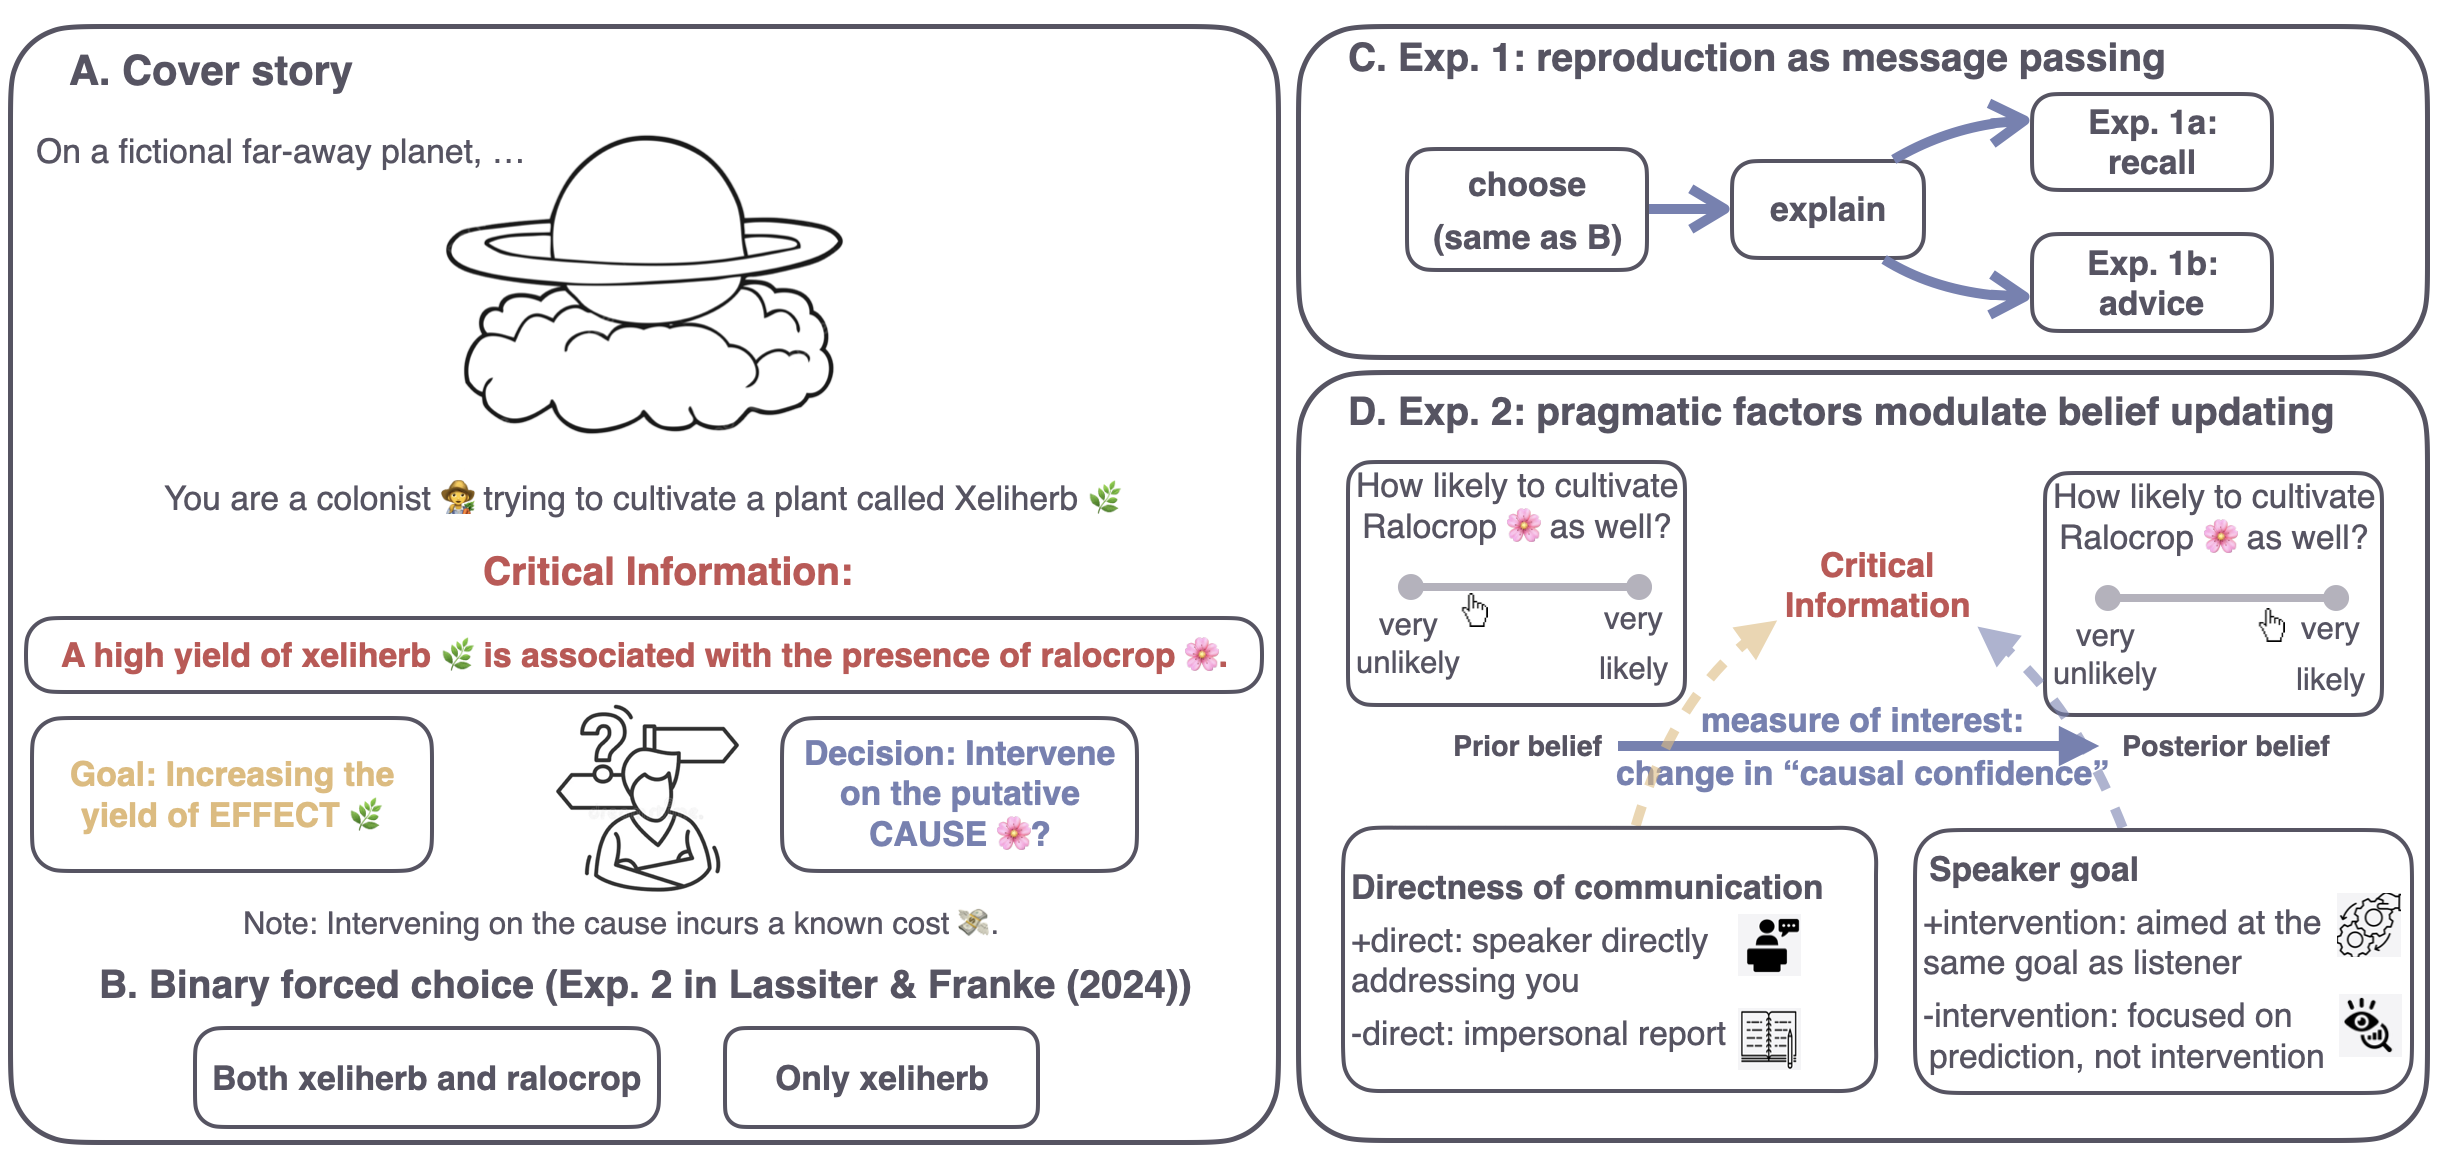
\includegraphics[width=0.78\linewidth]{figures-exp2/xeliherb_overview.png}
\end{center}
\vspace{0.2em}
\begin{minipage}[t]{0.31\linewidth}
  \proxybox{Action proxy}{choosing both plants means acting on the putative cause.}
\end{minipage}\hfill
\begin{minipage}[t]{0.31\linewidth}
  \proxybox{Language proxy}{causal paraphrases show how participants interpret the message.}
\end{minipage}\hfill
\begin{minipage}[t]{0.31\linewidth}
  \proxybox{Belief proxy}{prior-posterior slider change tracks causal belief updating.}
\end{minipage}
}

\begin{columns}
\column{0.5}

\block{Motivation and Accounts}{
\begin{itemize}
  \item Correlational statements can evoke causal interpretations and guide decisions, even without an explicit causal claim.
  \item We ask whether this enrichment reflects stable linguistic form or pragmatic reasoning about why the speaker used this message here.
\end{itemize}
\vspace{0.1em}
\begin{center}
\resizebox{0.90\linewidth}{!}{%
\begin{tikzpicture}[
  font=\small\sffamily,
  source/.style={
    rounded corners=5pt, draw=MainRed, line width=1.1pt,
    fill=MainRed!8, align=center, inner sep=7pt,
    text width=6.3in
  },
  account/.style={
    rounded corners=5pt, draw=DarkBlue, line width=1pt,
    fill=Blue10, align=left, inner sep=6pt,
    text width=4.05in
  },
  flow/.style={-{Stealth[length=8pt,width=6pt]}, line width=1.3pt, color=DarkBlue}
]
\node[source] (claim) {\textbf{Correlational Statement}\\ ``$X$ is associated with $Y$'' in a decision context};
\node[account, below=0.34in of claim, xshift=-2.16in] (struct) {
  \textcolor{MainRed}{\textbf{Structural bias}}\\
  Form + causal salience $\rightarrow$ similar readings across contexts.
};
\node[account, below=0.34in of claim, xshift=2.16in] (prag) {
  \textcolor{MainRed}{\textbf{Pragmatic inference}}\\
  Why say this here? Speaker, audience, and goal $\rightarrow$ different readings.
};
\draw[flow] (claim.south west) -- (struct.north);
\draw[flow] (claim.south east) -- (prag.north);
\end{tikzpicture}
}%
\end{center}
\vspace{-0.4em}
}

\block{Experiment 1: Message Passing}{
\begin{minipage}[t]{0.47\linewidth}
  \vspace{0pt}
  \studyfacts{%
    \factrow{Sample}{$N=99$}
    \factrow{Task}{1a: recall report; 1b: advise outpost}
    \factrow{Coding}{responses coded \textit{causal} / \textit{neutral} / \textit{none}}
  }
\end{minipage}\hfill
\begin{minipage}[t]{0.48\linewidth}
  \vspace{0pt}
  \begingroup
  \setlength{\fboxsep}{7pt}%
  \noindent\fcolorbox{MainRed!35}{MainRed!3}{%
    \begin{minipage}{0.91\linewidth}
      \RaggedRight
      \headline{Result:} Participants who chose both plants produced more causal paraphrases, especially when advising another outpost.\par\vspace{0.2em}
      {\small \headline{Model check:} the both-vs-only contrast was credibly positive in both recall and advice.}
    \end{minipage}%
  }%
  \endgroup
\end{minipage}
\vspace{0.4em}
\begin{center}
  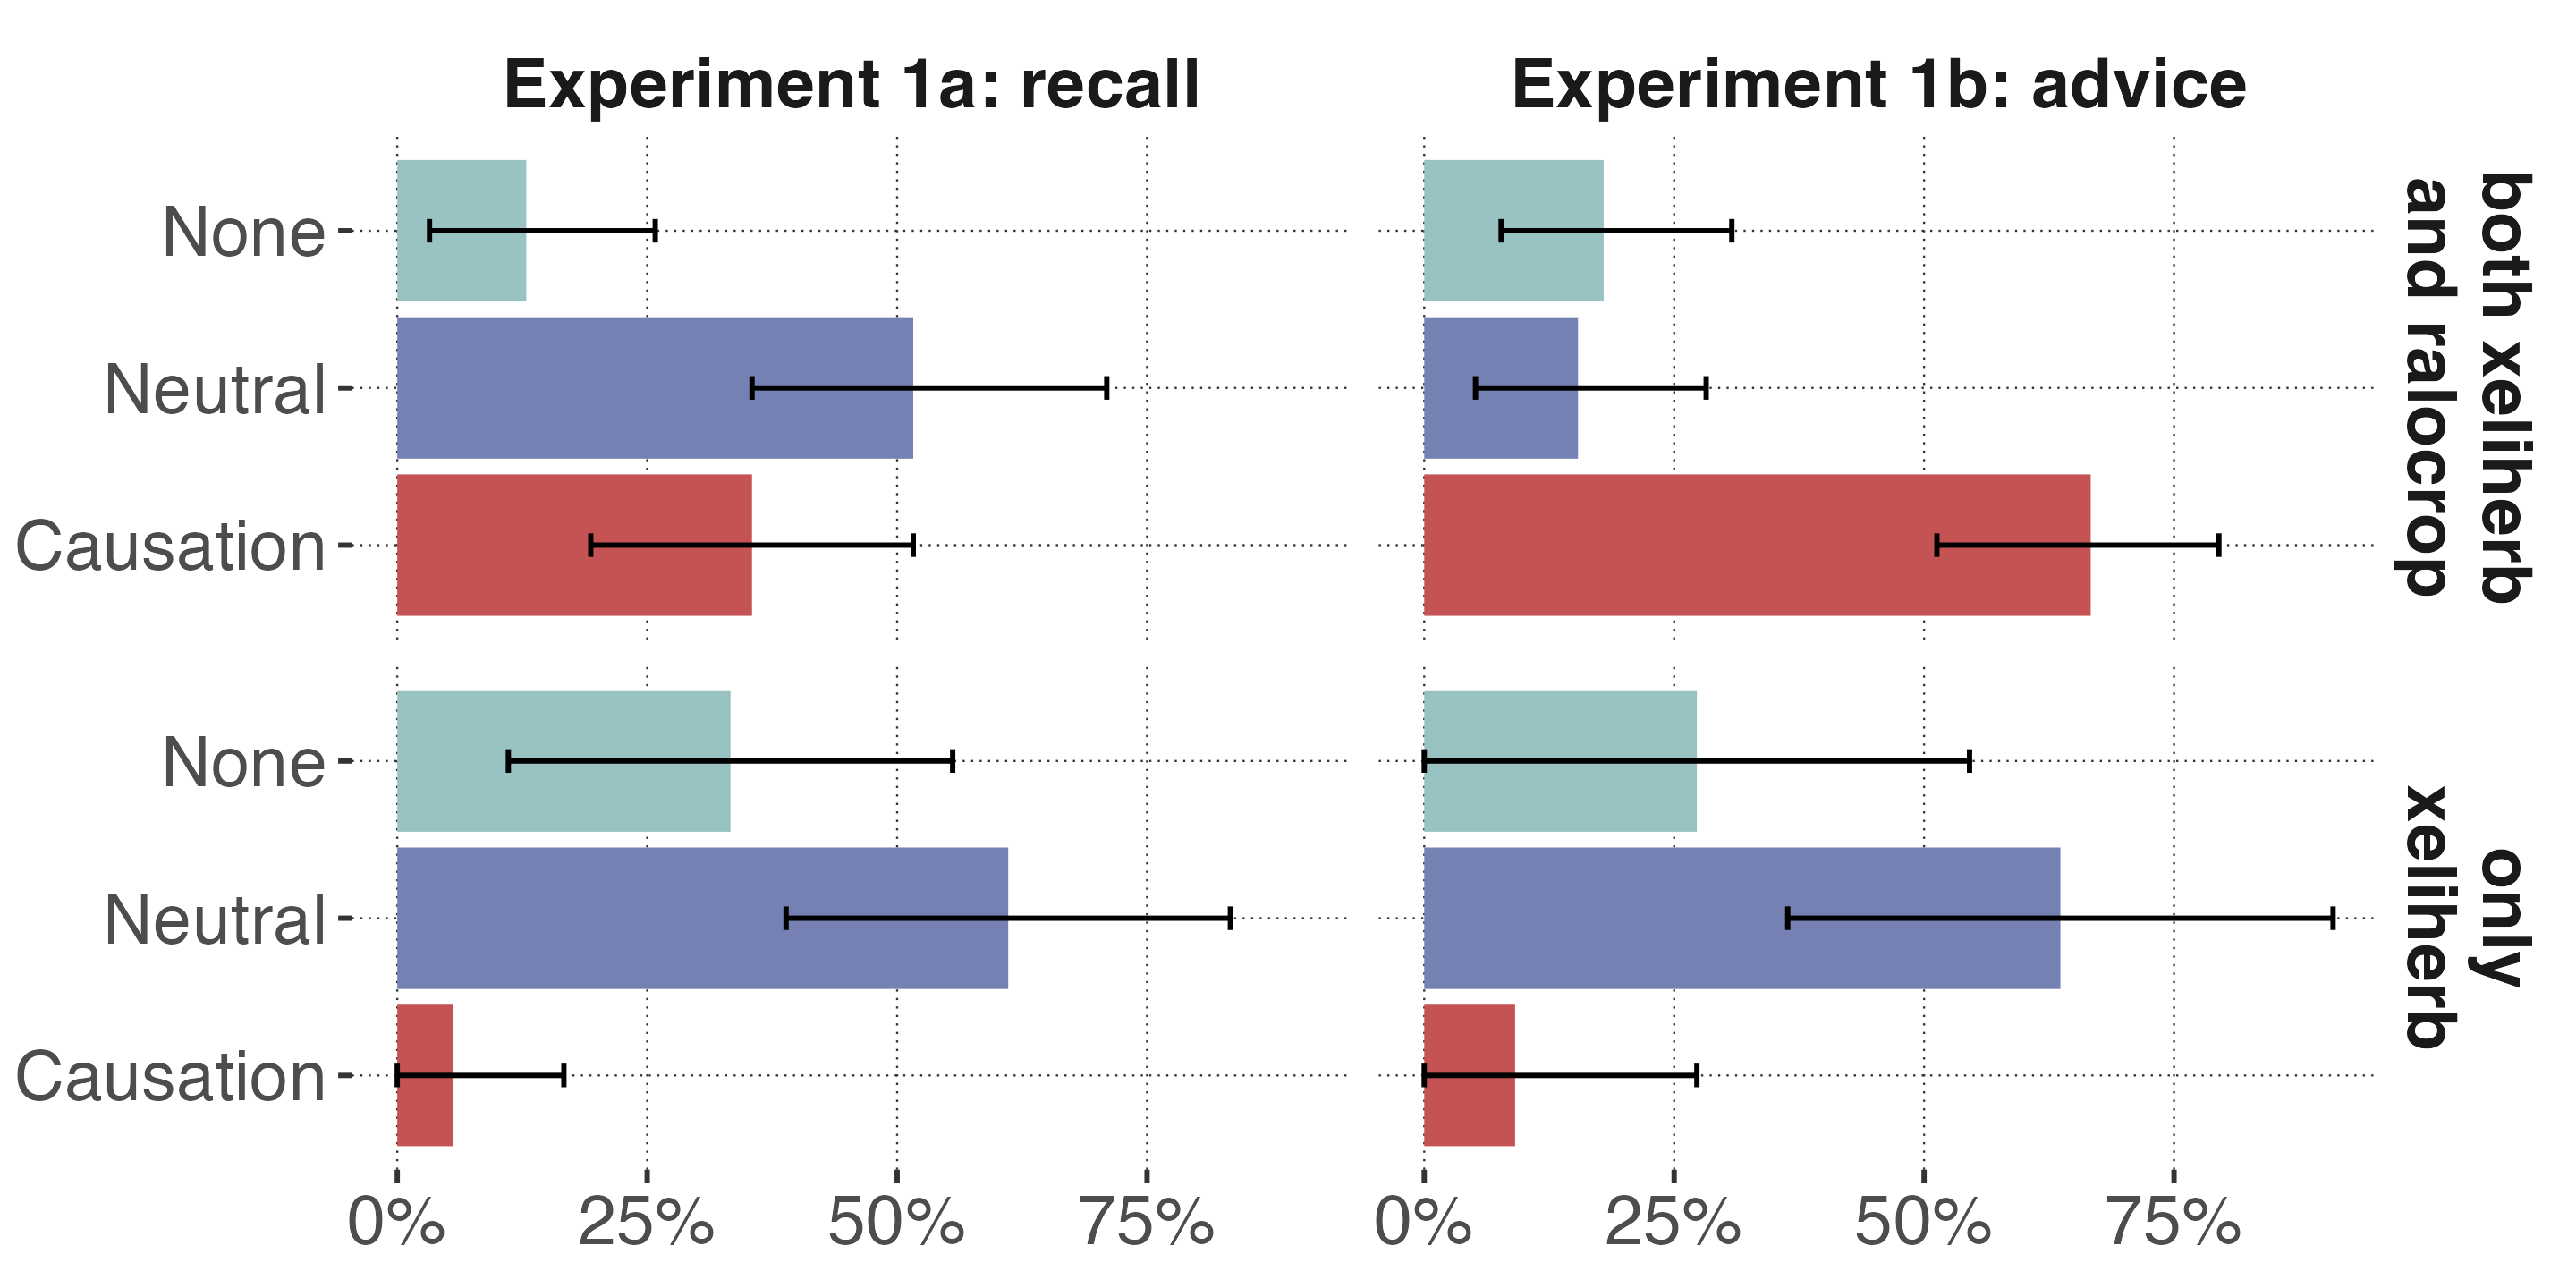
\includegraphics[width=0.9\linewidth]{figures-exp2/results_exp2_combined.png}
\end{center}
}

\block{}{
\begin{center}
  \textbf{References and Acknowledgments}
\end{center}
\vspace{-0.7em}
\begin{minipage}[t]{0.66\linewidth}
  \vspace{0pt}
  \setlength{\multicolsep}{0pt}
  \setlength{\columnsep}{0.9em}
  \nocite{lassiter2024rationality,gershman_causal_2023,goodman2016pragmatic,SperberWilson1995,adams2017readers,seifert2022causal}
  \begin{multicols}{2}
    \printbibliography[heading=none]
  \end{multicols}
\end{minipage}\hfill
\begin{minipage}[t]{0.30\linewidth}
  \vspace{0pt}
  \scriptsize\RaggedRight
  This research is part of the \textit{Communicating Causality} project, supported by the UK Arts and Humanities Research Council (AH/Z507490/1, PI: Daniel Lassiter), the Deutsche Forschungsgemeinschaft (project ID 547376651, PI: Michael Franke), and LMBayes (Leibniz Collaborative Excellence 22-20, PI: Anton Benz).
\end{minipage}
}

\column{0.5}

\block{Experiment 2: Belief Updating}{
\begingroup
\setlength{\fboxsep}{6pt}
\setlength{\tabcolsep}{0.55em}
\noindent\fcolorbox{MainRed!35}{MainRed!3}{%
  \begin{minipage}{0.965\linewidth}
    \RaggedRight
    \begin{tabular}{@{}>{\RaggedRight\arraybackslash}p{0.14\linewidth}>{\RaggedRight\arraybackslash}p{0.42\linewidth}>{\RaggedRight\arraybackslash}p{0.34\linewidth}@{}}
      \headline{Sample}\par $N=404$ &
      \headline{Procedure}\par prior rating $\rightarrow$ report $\rightarrow$ posterior rating &
      \headline{Measure}\par change: \mbox{posterior $-$ prior}
    \end{tabular}
  \end{minipage}%
}
\endgroup
\vspace{0.25em}
\begin{center}
  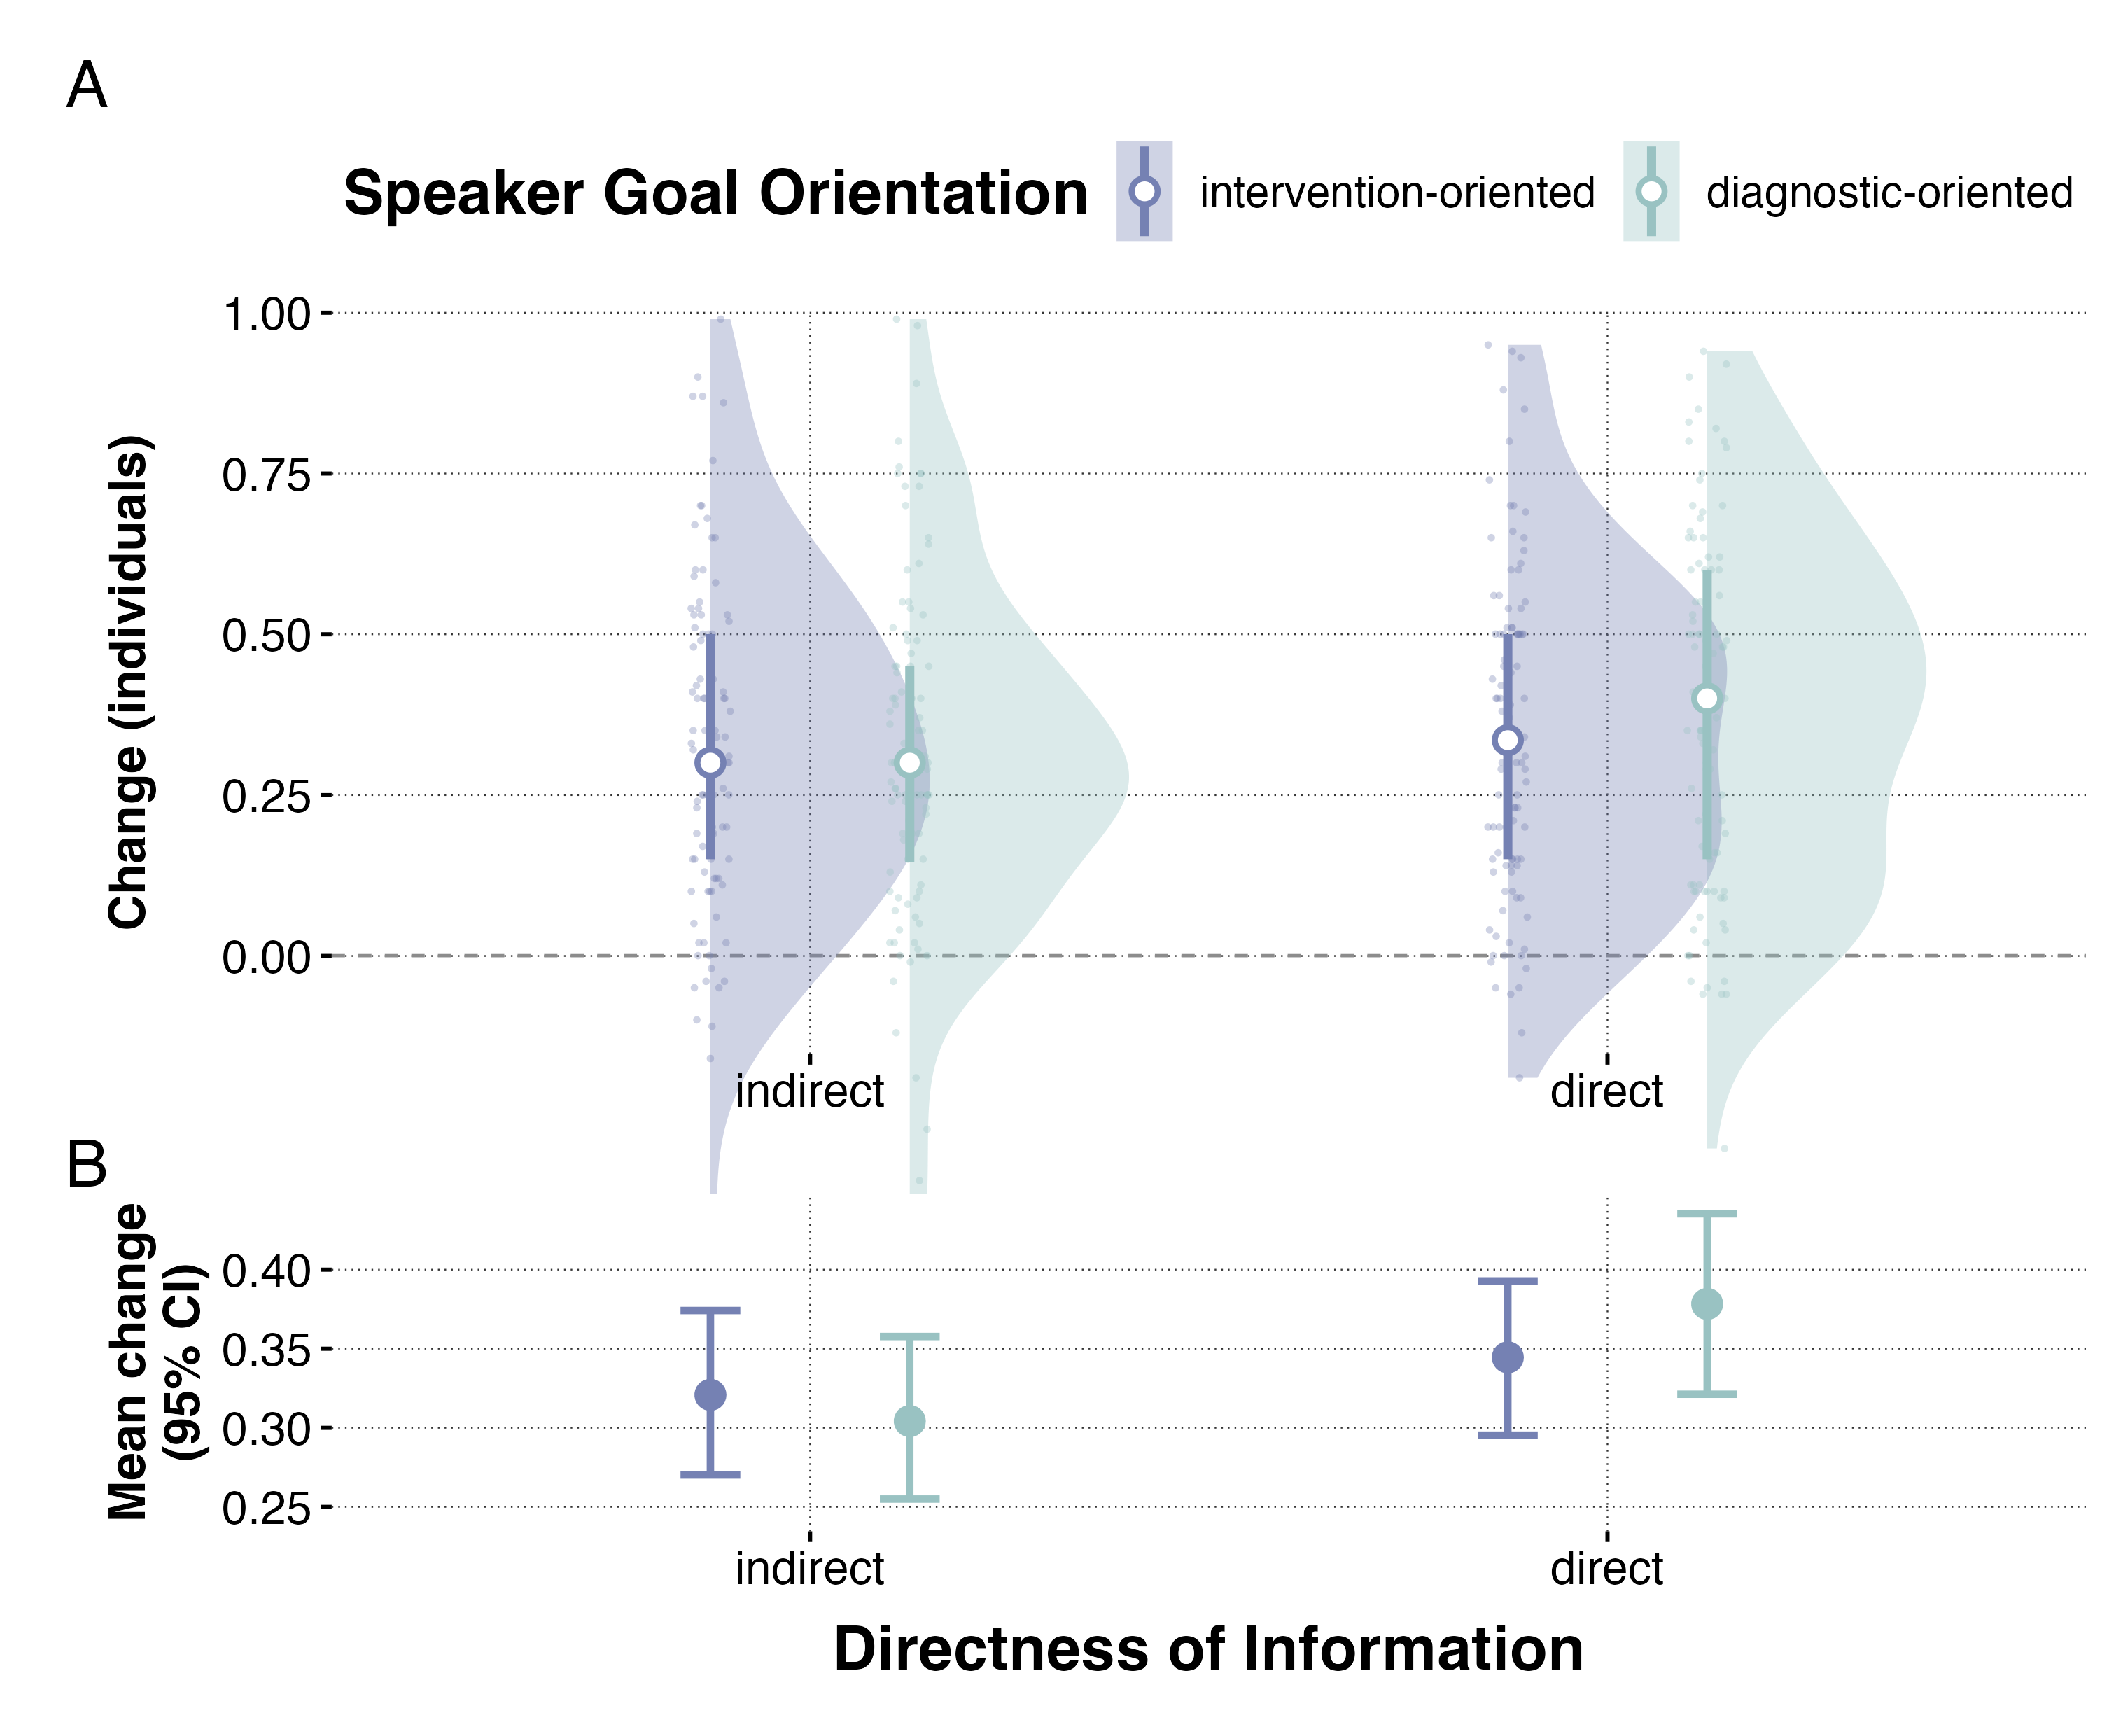
\includegraphics[width=0.9\linewidth]{figures-exp3/results_exp_3_individuals.png}
\end{center}
\vspace{0.2em}

\begingroup
\setlength{\fboxsep}{7pt}
\setlength{\tabcolsep}{0pt}
\noindent\fcolorbox{MainRed}{MainRed!4}{%
  \begin{minipage}{0.965\linewidth}
    \RaggedRight
    \headline{Design and pragmatic cues}\par\vspace{0.12em}
    \begin{tabular}{@{}>{\RaggedRight\arraybackslash}p{0.47\linewidth}>{\RaggedRight\arraybackslash}p{0.47\linewidth}@{}}
      \headline{Directness:} addressed report [evidence selected for this decision] vs. impersonal old note [archival evidence; weak audience design]. &
      \headline{Speaker goal:} cultivation team [intervention-oriented; improve farming] vs. localization team [diagnostic-oriented; locate \plant{xeliherb}].
    \end{tabular}
  \end{minipage}%
}
\endgroup
\par\vspace{0.3em}

\begingroup
\setlength{\fboxsep}{6pt}
  \noindent\fcolorbox{MainRed!35}{MainRed!3}{%
  \begin{minipage}{0.965\linewidth}
    \RaggedRight
    \headline{Result:} The correlational report generally increased willingness to intervene on the putative cause. Pragmatic context modulated the size of this update: in direct reports, belief increased more when the speaker's goal was not intervention-aligned, consistent with pragmatic reasoning about why this speaker chose this message for this audience; in indirect reports, the goal difference was small and tended toward the explicitly intervention-aligned farming context.\par\vspace{0.14em}
    {\small \headline{Model check:} overall posterior-minus-prior change was $+0.31$ [0.28, 0.34] on the 0--1 rating scale. Direct reports added $+0.06$ [0.02, 0.09], and the directness-by-goal interaction was credible ($+0.07$, $P=.97$).}
  \end{minipage}%
}
\endgroup
}

\block{Conclusion}{
\begin{itemize}
  \item \headline{Correlational information shifted causal belief:} willingness to intervene increased after the correlational message.
  \item \headline{Pragmatic context mattered:} audience design and speaker goals modulated causal belief updating.
\end{itemize}
}

\end{columns}
\end{document}
